% =============================================================================
% Plantilla de paper — Laboratorio 4: Capa de Red (OMNeT++)
% Cátedra de Redes y Sistemas Distribuidos — FaMAF/UNC
%
% Compilación:
%   pdflatex lab4-paper.tex
%   pdflatex lab4-paper.tex
%
% Carpeta figuras/: coloque ahí PDF/PNG exportados desde OMNeT++ o scripts.
% Antes de entregar: elimine todas las cajas \guia{...} y reemplace los
% textos de ejemplo por su contenido definitivo. Objetivo final: 6 a 8 páginas.
% =============================================================================

\documentclass[10pt,letterpaper,twocolumn]{article}

\usepackage[T1]{fontenc}
\usepackage[utf8]{inputenc}
\usepackage[english]{babel}
\usepackage[margin=0.9in]{geometry}
\usepackage{amsmath,amsfonts}
\usepackage{graphicx}
\usepackage{booktabs}
\usepackage{multirow}
\usepackage{subcaption}
\usepackage{xcolor}
\usepackage{url}
\usepackage[hidelinks]{hyperref}
\usepackage{tikz}
\usepackage{pgfplots}
\pgfplotsset{compat=1.18}
\usetikzlibrary{arrows.meta}

% ---------------------------------------------------------------------------
% Caja de instrucciones para el alumno (eliminar antes de la entrega final)
% ---------------------------------------------------------------------------
\newcommand{\guia}[1]{%
  \par\smallskip\noindent
  \fcolorbox{blue!60!black}{blue!4}{%
    \parbox{\dimexpr\linewidth-2\fboxsep-2\fboxrule}{%
      \small
      \textbf{\textcolor{blue!60!black}{Guía para completar:}}~#1
    }%
  }%
    \smallskip\par
}

% Tablas que deben caber dentro de una columna (formato 2 columnas)
\newcommand{\coltablesetup}{%
  \scriptsize
  \setlength{\tabcolsep}{3pt}%
  \renewcommand{\arraystretch}{1.08}%
}

% Datos del grupo — modifique estos campos
\newcommand{\Titulo}{Routing Strategies for Ring and General Topologies in OMNeT++}
\newcommand{\Grupo}{Grupo 31}
\newcommand{\Integrantes}{Bosque, Lissandro; Galassi, Franco; Pairetti, Joaquín}
\renewcommand{\refname}{Referencias}
\renewcommand{\abstractname}{Abstract}
\renewcommand{\appendixname}{Ap\'{e}ndice}

% Entorno estilo revista para metadatos en inglés
\newenvironment{IEEEkeywords}{%
  \smallskip\noindent\textbf{Index Terms---}%
}{\par\smallskip}

\begin{document}

\twocolumn[
\begin{@twocolumnfalse}
  \begin{center}
    {\LARGE\bfseries \Titulo\par}
    \vspace{0.6em}
    {\normalsize \Integrantes\par}
    \vspace{0.4em}
    {\small \Grupo, Facultad de Matemática, Astronomía, Física y Computación (FaMAF)\\
    Universidad Nacional de Córdoba, Argentina\par}
    \vspace{1em}
  \end{center}

  \begin{abstract}
  \noindent
  We analyze and redesign the routing layer of an 8-node ring network simulated
  in OMNeT++. We first characterize the kickstarter baseline, which always
  forwards through interface \texttt{lnk[0]} (clockwise), under two traffic
  scenarios: two sources and seven concurrent sources sending towards a common
  destination. Both scenarios show that this fixed rule concentrates all
  traffic on a single direction of the ring, leaving half of the link capacity
  idle and creating a saturated merge point ($\rho \approx 2$) in the light
  scenario, and a single converging bottleneck ($\rho \approx 7$) with an
  empirical stability threshold near \texttt{interArrivalTime} $\approx 7$\,s in
  the heavy one. We then design a distance-vector-style algorithm in which
  every node periodically floods small \texttt{HELLO} control packets in both
  directions; nodes use the hop count carried by these packets to build a local
  routing table and forward data through whichever interface yields the
  shortest known path, falling back to the kickstarter rule while the table is
  still converging. Re-running both scenarios with identical traffic, channels
  and random seed shows reductions of about 87\% in mean delay and 91\% in peak
  buffer occupancy for the light scenario, an exact doubling of sustained
  throughput in the heavy one (199 vs.\ 398 delivered packets in 200\,s), and a
  drop in the empirical stability threshold from $\approx$7\,s to
  $\approx$4--5\,s. No routing loops were observed in any run, a direct
  consequence of a HELLO-forwarding rule that is loop-free by construction on a
  ring. We close by discussing, conceptually, how the approach would need to
  change to generalize to arbitrary topologies (e.g.\ a star network) and how
  it would tolerate node failures -- both left as future work.
  \end{abstract}

  \begin{IEEEkeywords}
  Network simulation, OMNeT++, routing, ring topology, performance evaluation,
  queueing, stability.
  \end{IEEEkeywords}

  \vspace{0.5em}
\end{@twocolumnfalse}
]

\selectlanguage{english}
% Contenido principal en español (sin babel-spanish; títulos de sección en español manualmente)

\section{Introducción}
\label{sec:intro}

Este artículo reporta el análisis y diseño de estrategias de enrutamiento
implementadas sobre el modelo de red del Laboratorio~4. Fue desarrollado por el grupo de forma tal que se priorizó la discusión total
de su contenido, para luego dividir los temas y que cada integrante redacte un texto base para luego
compartirlo a los demás. Por último, se hizo una revisión y corrección de errores.

A través de un \textit{kickstarter}, provisto por la cátedra de Redes 2026, nos fue dada una implementación base
de un modelo de red de 8 nodos conectados en forma de anillo 
con el objetivo de que la misma fuera analizada en OMNeT++ para lograr 
una mejor comprensión del tráfico de red en el modelo base con unas métricas iniciales
y así plantear una forma más óptima de enviar los paquetes
implementando cambios en el modelo para lograr el enrutamiento deseado. 
En el \textit{kickstarter} , con el enrutamiento inicial todos los paquetes son enviados en 
sentido horario a partir de \texttt{toLnk[0]} hasta llegar a su destino, 
ignorando si se tarda más que enviarlo en sentido antihorario. 
Por ejemplo, si se tuviése un paquete en el nodo cero, y se quisiera enviarlo hasta el 5, con el modelo inicial
se recorrerían 5 nodos. En cambio, si se hiciera con el modelo modificado, se compararía su distancia con el sentido antihorario, 
el cuál resultaría más eficiente, ya que recorrería 3 nodos.


Resumiendo, el modelo modificado busca cual es la distancia de un nodo a otro en sentido horario y antihorario,
decide cual es menor, por lo tanto más eficiente, y recorre los nodos en ese sentido.

\section{Escenario y modelo de simulación}
\label{sec:modelo}

\subsection{Topología y configuración de tráfico}

\begin{figure}[!h]
  \centering
  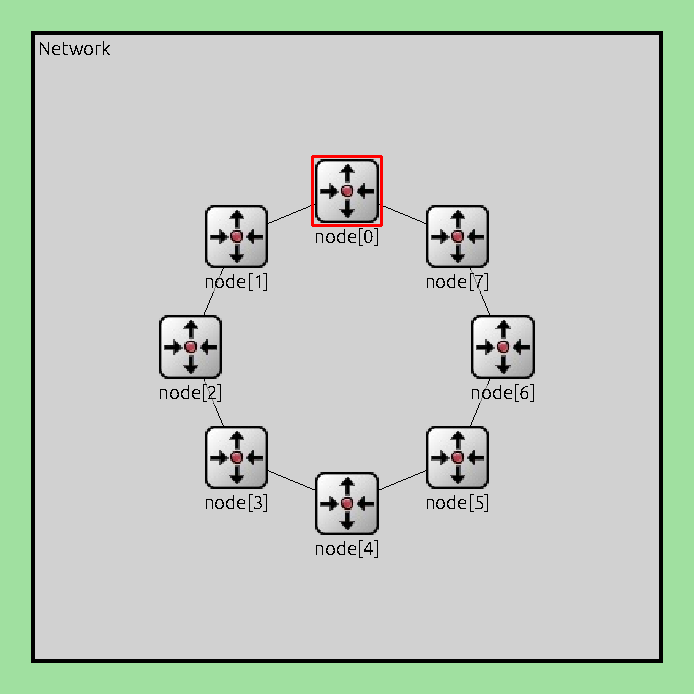
\includegraphics[width=\linewidth]{figuras/topologia-anillo.pdf}
  \caption{Topología en anillo de 8 nodos graficada en OMNeT++.}
  \label{fig:topologia}
\end{figure}

El modelo consiste en una red en forma de anillo de 8 nodos implementada en OMNeT++.
Cada nodo se conecta con sus dos vecinos mediante enlaces \textit{full-duplex}
(bidireccionales) de 1\,Mbps de capacidad y 100\,µs de delay, formando un
anillo cerrado. Los nodos se indexan del 0 al 7; el nodo \texttt{node[1]}
tiene como vecinos a \texttt{node[0]} (interfaz \texttt{lnk[0]}) y a
\texttt{node[2]} (interfaz \texttt{lnk[1]}), y así sucesivamente.

Internamente, cada nodo está compuesto por tres capas:
\begin{itemize}
  \item \textbf{Capa de aplicación} (\texttt{app}): genera paquetes con un
  tamaño configurable (\texttt{packetByteSize}) a intervalos aleatorios
  distribuidos exponencialmente (\texttt{interArrivalTime}), y registra la
  demora extremo a extremo de los paquetes recibidos.
  \item \textbf{Capa de red} (\texttt{net}): recibe paquetes desde \texttt{app}
  o desde las capas de enlace, y decide por qué interfaz reenviarlos según
  el algoritmo de enrutamiento implementado.
  \item \textbf{Capas de enlace} (\texttt{lnk[0]} y \texttt{lnk[1]}): modelan
  un buffer de salida y el canal físico hacia cada vecino.
\end{itemize}

Como muestra la Fig.~\ref{fig:topologia}, el tráfico puede circular en sentido
horario (por \texttt{lnk[0]}) o antihorario (por \texttt{lnk[1]}). El kickstarter utiliza siempre \texttt{lnk[0]},
independientemente del destino.

Se definen dos escenarios de tráfico, resumidos en la
Tabla~\ref{tab:config}:

\begin{itemize}
  \item \textbf{Caso 1}: \texttt{node[0]} y \texttt{node[2]} transmiten
  paquetes hacia \texttt{node[5]}.
  \item \textbf{Caso 2}: los 7 nodos restantes (0--4, 6--7) transmiten
  simultáneamente hacia \texttt{node[5]} con los mismos parámetros de tráfico.
\end{itemize}

\begin{table}[!ht]
  \centering
  \caption{Configuración experimental por escenario.}
  \label{tab:config}
  \coltablesetup
  \resizebox{\columnwidth}{!}{%
  \begin{tabular}{@{}lccc@{}}
    \toprule
     & \textbf{Caso 1} & \textbf{Caso 2} & \textbf{Comparación} \\
    \midrule
    Fuentes activas & \texttt{n[0]}, \texttt{n[2]} & 7 $\to$ \texttt{n[5]} & 1 y 2 \\
    Destino & \texttt{n[5]} & \texttt{n[5]} & \texttt{n[5]} \\
    \texttt{packetByteSize} (B) & 125000 & 125000 & 125000 \\
    \texttt{interArrivalTime} & \texttt{exp(1)} & \texttt{exp(1)} & \texttt{exp(1)} \\
    T. simulación (s) & 200 & 200 & 200 \\
    Semilla & 0 & 0 & 0 \\
    \bottomrule
  \end{tabular}%
  }
\end{table}

\subsection{Métricas registradas}

Se instrumentaron las siguientes métricas en el modelo:

\begin{itemize}
  \item \textbf{Demora extremo a extremo}: tiempo transcurrido desde que un
  paquete es generado en la capa de aplicación del nodo origen hasta que es
  entregado en el nodo destino. Registrada como vector y escalar en
  \texttt{app}.
  \item \textbf{Cantidad de saltos}: número de nodos intermedios que atraviesa
  cada paquete. Se incrementa en cada paso por la capa \texttt{net} y se
  registra al llegar al destino.
  \item \textbf{Ocupación del buffer}: cantidad de paquetes en espera en cada
  \texttt{lnk}, registrada como vector temporal. Permite identificar
  saturación en enlaces específicos.
  \item \textbf{Utilización del enlace}: fracción del tiempo en que el canal
  estuvo ocupado transmitiendo. Calculada en cada \texttt{lnk} como escalar
  al final de la simulación.
\end{itemize}

\begin{table}[!ht]
  \centering
  \caption{Métricas instrumentadas en el simulador.}
  \label{tab:metricas}
  \coltablesetup
  \resizebox{\columnwidth}{!}{%
  \begin{tabular}{@{}lcc@{}}
    \toprule
    \textbf{Métrica} & \textbf{Módulo} & \textbf{Unidad} \\
    \midrule
    Demora E2E         & \texttt{app}            & s \\
    Saltos/paquete     & \texttt{net} / \texttt{app} & adim. \\
    Ocupación buffer   & \texttt{lnk[0..1]}      & pkts \\
    Utilización enlace & \texttt{lnk[0..1]}      & adim.\ ($[0,1]$) \\
    \bottomrule
  \end{tabular}
  }
\end{table}

\section{Tarea de análisis: evaluación del kickstarter}
\label{sec:analisis}

\subsection{Caso 1: tráfico configurado (\texttt{node[0]} y \texttt{node[2]} $\rightarrow$ \texttt{node[5]})}

Bajo la configuración por defecto del kickstarter (Tabla~\ref{tab:config},
columna ``Caso 1''), \texttt{node[0]} y \texttt{node[2]} generan tráfico hacia
\texttt{node[5]} a una tasa media de un paquete por segundo cada uno
(\texttt{exponential(1)}), con paquetes de 125000\,B que insumen exactamente 1
segundo de transmisión por enlace (a 1\,Mbps). La Tabla~\ref{tab:caso1} resume
las cuatro métricas instrumentadas al cabo de 200\,s de simulación.

La demora media observada fue de 51.16\,s (máximo 105.56\,s, desviación
28.31\,s), y cada paquete recorrió en promedio 3.92 saltos --- un valor muy
cercano al máximo posible de 5, que es justamente la distancia \emph{en sentido
horario} entre \texttt{node[2]} y \texttt{node[5]}. Esto ya sugiere que el
algoritmo no usa el camino más corto disponible: en sentido antihorario,
\texttt{node[2]} llegaría a \texttt{node[5]} en sólo 3 saltos
(\texttt{2}$\to$\texttt{3}$\to$\texttt{4}$\to$\texttt{5}).

La Fig.~\ref{fig:caso1-demora} grafica la utilización de cada interfaz de cada
nodo y deja ver con claridad que \emph{todo} el tráfico circula por
\texttt{lnk[0]} (sentido horario): los cinco nodos del arco que va de
\texttt{node[2]} a \texttt{node[5]} pasando por \texttt{node[0]} ---es decir
\texttt{node[2]}, \texttt{node[1]}, \texttt{node[0]}, \texttt{node[7]} y
\texttt{node[6]}--- presentan utilizaciones de \texttt{lnk[0]} entre 93.5\% y
99.5\%, mientras que las 16 interfaces \texttt{lnk[1]} de la red permanecen en
0\%. La gran desviación de la utilización de enlace que muestra la
Tabla~\ref{tab:caso1} (44.9 puntos porcentuales sobre un promedio de apenas
30.3\%) es la huella numérica de esa asimetría: la mitad de la capacidad de la
red --- el sentido antihorario completo --- queda ociosa.

El enlace más cargado es \texttt{node[0].lnk[0]}, con 99.5\% de utilización. No
es casualidad: es el punto donde confluyen los dos flujos, ya que el camino
horario de \texttt{node[2]} (\texttt{2}$\to$\texttt{1}$\to$\texttt{0}$\to$%
\texttt{7}$\to$\texttt{6}$\to$\texttt{5}, 5 saltos) pasa por \texttt{node[0]}
antes de seguir junto con el tráfico que \texttt{node[0]} genera para sí mismo.
La carga ofrecida sobre ese enlace es entonces, en régimen, la suma de ambas
fuentes ($\rho \approx 2\lambda = 2$ paquetes/s), el doble de lo que puede
servir (1 paquete/s, fijado por \texttt{packetByteSize} y la tasa del canal).
El resultado es una cola que crece de forma sostenida durante toda la
simulación --- de 0 a 190 paquetes en 200\,s, con una ocupación media de 91.3
(Tabla~\ref{tab:caso1}) --- sin alcanzar nunca un régimen estacionario.

En síntesis: los recursos se usan de forma muy desigual (la mitad de los
enlaces ociosos, y en el otro extremo un punto de fusión saturado al doble de
su capacidad), y claramente \emph{se puede mejorar}: alcanzaría con decidir el
sentido de envío según la distancia real al destino en lugar de hacerlo siempre
en sentido horario. Esa es la idea central del algoritmo que presentamos en la
Sección~\ref{sec:diseno}.

\begin{table}[!ht]
  \centering
  \caption{Resultados del Caso~1 (baseline kickstarter, 200\,s, semilla 0). La
  fila ``Ocupación buffer'' corresponde al enlace más cargado
  (\texttt{node[0].lnk[0]}); ``Util.\ enlace'' resume la distribución de
  utilización entre las 16 interfaces de la red.}
  \label{tab:caso1}
  \coltablesetup
  \resizebox{\columnwidth}{!}{%
  \begin{tabular}{@{}lrrr@{}}
    \toprule
    \textbf{Métrica} & \textbf{Prom.} & \textbf{Máx.} & \textbf{Desv.} \\
    \midrule
    Demora (s)        & 51.16 & 105.56 & 28.31 \\
    Saltos            & 3.92  & 5      & 1.00  \\
    Ocupación buffer (\texttt{n[0].lnk[0]}, pkts) & 91.28 & 190 & 54.83 \\
    Util. enlace (\%, las 16 interfaces) & 30.3 & 99.5 & 44.9 \\
    \bottomrule
  \end{tabular}%
  }
\end{table}

\begin{figure}[!t]
  \centering
  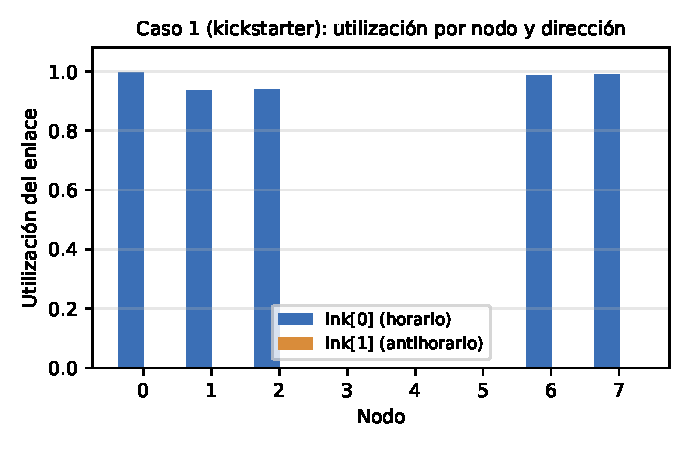
\includegraphics[width=\linewidth]{figuras/fig-caso1-utilizacion.pdf}
  \caption{Caso 1 (kickstarter): utilización de \texttt{lnk[0]} (horario) y
  \texttt{lnk[1]} (antihorario) en cada nodo. Todo el tráfico de ambos flujos
  circula por \texttt{lnk[0]}; las 16 interfaces \texttt{lnk[1]} quedan en 0\%.}
  \label{fig:caso1-demora}
\end{figure}

\subsection{Caso 2: tráfico sostenido hacia \texttt{node[5]}}
\label{sec:caso2}

Activamos ahora las siete fuentes restantes (\texttt{node[0]} a
\texttt{node[4]}, \texttt{node[6]} y \texttt{node[7]}, columna ``Caso 2'' de la
Tabla~\ref{tab:config}) con los mismos parámetros que en el Caso 1
(\texttt{interArrivalTime} medio de 1\,s, paquetes de 125000\,B), todas hacia
\texttt{node[5]}.

Bajo esta configuración la red queda claramente sobrecargada: la demora media
subió a 64.53\,s (máximo 184.23\,s, desviación 44.0\,s), y en 200\,s sólo se
entregaron 199 de los cerca de 1400 paquetes que generan siete fuentes a
$\approx$1\,paquete/s. Los enlaces \texttt{node[6].lnk[0]} y
\texttt{node[7].lnk[0]} --- los dos últimos saltos del camino horario hacia
\texttt{node[5]} --- llegan a 100\% de utilización, con colas que en promedio
rondan los 82 y 99 paquetes (máximos de 164 y 205) y que, igual que en el Caso
1, no dejan de crecer dentro de la ventana simulada. El número de saltos
promedio bajó a 2.06 (máximo 7, la vuelta completa al anillo) simplemente
porque ahora hay fuentes mucho más cerca de \texttt{node[5]} ---
\texttt{node[4]} está a un solo salto en sentido horario---, no porque el
algoritmo haya cambiado su forma de elegir camino.

Para saber si este comportamiento depende de la intensidad del tráfico o es
estructural, barrimos sistemáticamente \texttt{interArrivalTime} sobre el
conjunto $\{2,3,4,5,6,7,8,10,15,20\}$\,s (200\,s de simulación por punto,
configuración \texttt{Caso2Sweep} del \texttt{omnetpp.ini}). Como el modelo no
descarta paquetes --- los buffers de \texttt{Lnk} son colas \texttt{cQueue}
sin límite de tamaño ---, no existe una columna de ``pérdidas'' propiamente
dicha; en su lugar caracterizamos la estabilidad con la \emph{pendiente} de la
ocupación del buffer del enlace más cargado (\texttt{node[6].lnk[0]}, por el
que pasan los siete flujos) a lo largo de la corrida, estimada por regresión
lineal sobre la serie temporal registrada: una pendiente cercana a cero indica
que la cola converge a un régimen estacionario, y una pendiente claramente
positiva indica que crece sin cota dentro de la ventana observada. La
Tabla~\ref{tab:caso2-sweep} resume los resultados, y la
Fig.~\ref{fig:caso2-estabilidad} grafica la demora media resultante (junto con
la curva del algoritmo propuesto, que se compara en la
Sección~\ref{sec:evaluacion}).

\begin{table}[!ht]
  \centering
  \caption{Caso 2: demora media, ocupación media de \texttt{node[6].lnk[0]} y
  pendiente de su crecimiento vs.\ \texttt{interArrivalTime} (200\,s/punto).
  ``Estab.'' = Sí cuando la pendiente es $\approx$0 (cola acotada).}
  \label{tab:caso2-sweep}
  \coltablesetup
  \resizebox{\columnwidth}{!}{%
  \begin{tabular}{@{}rrrrc@{}}
    \toprule
    \textbf{\texttt{interArriv.} (s)} & \textbf{Demora (s)} & \textbf{Cola (pkts)} & \textbf{Pend. (pkts/s)} & \textbf{Estab.} \\
    \midrule
    2  & 56.90 & 39.30 & $+0.42$ & No \\
    3  & 48.93 & 29.98 & $+0.36$ & No \\
    4  & 44.71 & 26.68 & $+0.22$ & No \\
    5  & 39.84 & 21.66 & $+0.20$ & No \\
    6  & 23.13 & 11.55 & $+0.15$ & No \\
    7  &  7.16 &  1.29 & $+0.01$ & Límite \\
    8  &  5.56 &  0.46 & $+0.00$ & Sí \\
    10 &  4.71 &  0.24 & $-0.00$ & Sí \\
    15 &  4.31 &  0.05 & $\approx0$ & Sí \\
    20 &  4.33 &  0.01 & $\approx0$ & Sí \\
    \bottomrule
  \end{tabular}%
  }
\end{table}

\begin{figure}[!t]
  \centering
  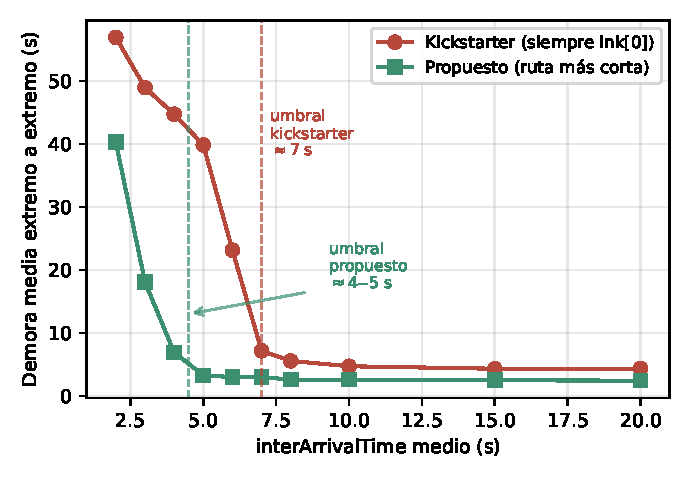
\includegraphics[width=\linewidth]{figuras/fig-caso2-estabilidad.pdf}
  \caption{Demora media extremo a extremo vs.\ \texttt{interArrivalTime} medio
  para el Caso 2, kickstarter y algoritmo propuesto (Sección~\ref{sec:diseno}).
  Las líneas punteadas marcan el umbral de estabilidad estimado de cada uno.}
  \label{fig:caso2-estabilidad}
\end{figure}

Se observa una transición neta entre \texttt{interArrivalTime} = 6\,s
(pendiente $+0.15$ paquetes/s, cola todavía en franco crecimiento) y 8\,s
(pendiente prácticamente nula). \textbf{Concluimos que la red permanece estable
a partir de \texttt{interArrivalTime} $\approx$ 7\,s}: ese es el punto en que
la tasa de servicio del cuello de botella (1 paquete/s, fijada por
\texttt{packetByteSize} y la tasa del canal) iguala la tasa agregada de llegada
de las siete fuentes que confluyen en él, $\lambda_{total} =
7/\texttt{interArrivalTime}$. El valor crítico teórico, $\rho =
\lambda_{total}/\mu = 1$, se alcanza exactamente en \texttt{interArrivalTime} =
7\,s; la corrida con ese valor exhibe justo el comportamiento esperado en el
punto crítico --- pendiente residual de apenas $+0.007$ paquetes/s, la cola
fluctúa mucho pero casi no crece en promedio ---, lo cual nos da bastante
confianza en que el modelo y la medición son consistentes con la teoría de
colas elemental ($M/M/1$, $\rho = \lambda/\mu$).

\section{Diseño del algoritmo de enrutamiento propuesto}
\label{sec:diseno}

\subsection{Información disponible y estructuras de datos}

Cada nodo dispone únicamente de la información que puede observar
\emph{localmente}: su propio identificador
(\texttt{getParentModule()->getIndex()}), la cantidad de interfaces que posee
(\texttt{gateSize("toLnk\$o")}) y los paquetes que recibe por cada una de
ellas. La consigna prohíbe usar \texttt{cTopology} o iteradores de
\texttt{cGate} para conocer la red de antemano, así que en el instante inicial
un nodo no sabe ni cuántos nodos hay en el anillo ni qué hay del otro lado de
sus enlaces.

Para resolver esto adoptamos un mecanismo de descubrimiento por
\emph{inundación de paquetes de control} tipo \texttt{HELLO} (en la línea de
los protocolos de vector de distancias): periódicamente
(\texttt{helloInterval}, 20\,s por defecto), cada nodo envía un paquete
\texttt{HELLO} pequeño --- 64\,B, frente a los 125000\,B de un paquete de
datos: una sobrecarga de control medida en $\approx 0.03\%$ de utilización de
enlace en nuestras corridas --- por \emph{cada} una de sus interfaces,
anunciando su propio identificador y un contador de saltos que arranca en 1
(formato en la Tabla~\ref{tab:hello}).

\begin{table}[!ht]
  \centering
  \caption{Campos relevantes del paquete de control \texttt{HELLO} (reutiliza
  la clase \texttt{Packet}, distinguido por \texttt{isHello = true}).}
  \label{tab:hello}
  \coltablesetup
  \resizebox{\columnwidth}{!}{%
  \begin{tabular}{@{}lll@{}}
    \toprule
    \textbf{Campo} & \textbf{Significado} & \textbf{Valor} \\
    \midrule
    \texttt{source}      & nodo que originó el HELLO     & \texttt{myId} \\
    \texttt{hopCount}    & saltos recorridos hasta ahora & 1, +1 por salto \\
    \texttt{destination} & no se usa en control          & $-1$ \\
    \texttt{byteLength}  & tamaño del paquete            & 64\,B \\
    \bottomrule
  \end{tabular}%
  }
\end{table}

La estructura central es una tabla de rutas local,
\texttt{std::map<int, Route>}, con \texttt{Route\{int outGate; int hopCount;\}},
que asocia cada identificador de destino \emph{conocido} con la interfaz de
salida y la distancia del mejor camino aprendido hacia él. La
Tabla~\ref{tab:rutas} muestra cómo luce esta tabla en \texttt{node[1]} una vez
que la red convergió (situación del Caso 2, Sección~\ref{sec:evaluacion}):
nótese el empate a 4 saltos hacia \texttt{node[5]}, resuelto --- por el orden
en que \texttt{node[1]} recibió los \texttt{HELLO} respectivos --- a favor de
\texttt{lnk[1]}, justo lo que se observó en la simulación.

\begin{table}[!ht]
  \centering
  \caption{Tabla de rutas de \texttt{node[1]} una vez convergido el descubrimiento.}
  \label{tab:rutas}
  \coltablesetup
  \resizebox{\columnwidth}{!}{%
  \begin{tabular}{@{}clc@{}}
    \toprule
    \textbf{Destino} & \textbf{Interfaz} & \textbf{Saltos} \\
    \midrule
    \texttt{node[0]} & \texttt{lnk[0]} & 1 \\
    \texttt{node[7]} & \texttt{lnk[0]} & 2 \\
    \texttt{node[6]} & \texttt{lnk[0]} & 3 \\
    \texttt{node[2]} & \texttt{lnk[1]} & 1 \\
    \texttt{node[3]} & \texttt{lnk[1]} & 2 \\
    \texttt{node[4]} & \texttt{lnk[1]} & 3 \\
    \texttt{node[5]} & \texttt{lnk[1]} & 4 $\leftarrow$ \textit{empate, ver texto} \\
    \bottomrule
  \end{tabular}%
  }
\end{table}

\subsection{Reglas de decisión}

El algoritmo combina dos mecanismos sencillos:

\begin{enumerate}
  \item \textbf{Aprendizaje de rutas.} Al recibir un \texttt{HELLO} por la
  interfaz $i$, originado en el nodo $s$ con contador de saltos $h$, el nodo
  registra ``puedo llegar a $s$ por $i$, a $h$ saltos'' y actualiza su tabla
  \emph{sólo si} ese camino es estrictamente más corto que el mejor que ya
  conocía (\texttt{learnRoute}). Luego reenvía el \texttt{HELLO}
  ---incrementando su contador--- por la interfaz \emph{opuesta} a la de
  llegada (\texttt{1 - i}). En un anillo, esto garantiza que cada \texttt{HELLO}
  recorra el anillo exactamente una vez en cada sentido y vuelva a su origen,
  momento en el que se descarta. No hace falta ningún mecanismo adicional
  (números de secuencia, TTL) para que la inundación termine: la propia regla
  ``seguir de largo por la interfaz opuesta'' es, en una topología circular,
  libre de bucles por construcción.
  \item \textbf{Reenvío de datos.} Al recibir un paquete cuyo destino no es el
  nodo local, se incrementa su contador de saltos (estadística \emph{Cantidad
  de saltos}, Sección~\ref{sec:modelo}) y se busca el destino en
  \texttt{routingTable}. Si hay una entrada, el paquete se reenvía por la
  interfaz indicada; si todavía no se aprendió ninguna ruta hacia ese destino
  ---algo que sólo puede ocurrir en los primerísimos instantes de la
  simulación, antes de que el primer \texttt{HELLO} complete su recorrido---,
  el nodo recurre al criterio del \emph{kickstarter} (\texttt{lnk[0]}) como
  valor por defecto, dándole tiempo al descubrimiento para converger.
\end{enumerate}

\begin{small}
\begin{verbatim}
al recibir HELLO por interfaz i, origen s, saltos h:
  si s == miId:
    descartar (dio toda la vuelta al anillo)
  sino:
    si no conozco ruta a s, o h < la conocida:
      tablaRutas[s] <- (interfaz = i, saltos = h)
    reenviar por interfaz (1 - i), con saltos = h+1

al recibir paquete de datos p:
  si destino(p) == miId:
    entregar a la capa de aplicacion
  sino:
    saltos(p) <- saltos(p) + 1
    si destino(p) en tablaRutas:
      j <- tablaRutas[destino(p)].interfaz
    sino:
      j <- 0   (criterio del kickstarter, mientras converge)
    reenviar p por interfaz j
\end{verbatim}
\end{small}

Reutilizamos la misma clase \texttt{Packet} para datos y control,
distinguiéndolos con el campo booleano \texttt{isHello} (Tabla~\ref{tab:hello}).
Esa decisión, de paso, nos hizo notar un error latente del \emph{kickstarter}:
\texttt{App.cc} usa el segundo argumento posicional del constructor de
\texttt{cMessage} --- que en realidad fija el \emph{kind} del mensaje --- para
otra cosa, así que distinguir \texttt{HELLO} de datos mediante
\texttt{setKind()}/\texttt{getKind()} (nuestro primer intento) producía
colisiones y caídas del simulador; el campo explícito \texttt{isHello} evita el
problema por completo.

\paragraph{Ejemplo numérico.} Consideremos un paquete generado en
\texttt{node[2]} con destino \texttt{node[5]} (el flujo del Caso 1 que más se
beneficia del cambio, Sección~\ref{sec:analisis}). Una vez convergidas las
tablas, \texttt{node[2]} sabe que \texttt{node[5]} está a 3 saltos por
\texttt{lnk[1]} (antihorario: \texttt{2}$\to$\texttt{3}$\to$\texttt{4}$\to$%
\texttt{5}) y a 5 por \texttt{lnk[0]}, así que reenvía por \texttt{lnk[1]}.
\texttt{node[3]} hace lo mismo: \texttt{node[5]} está a 2 saltos por su
\texttt{lnk[1]} y a 6 por su \texttt{lnk[0]}; reenvía hacia \texttt{node[4]}.
Finalmente \texttt{node[4]} ve que \texttt{node[5]} es su vecino directo (1
salto) y se lo entrega. El paquete recorre \texttt{node[2]} $\to$
\texttt{node[3]} $\to$ \texttt{node[4]} $\to$ \texttt{node[5]}: 3 saltos, en
lugar de los 5 que recorría con el kickstarter, y sin pasar nunca por el tramo
congestionado de la Fig.~\ref{fig:caso1-demora}. Es exactamente lo que se
observó en la simulación: con el algoritmo propuesto el conteo de saltos del
Caso 1 fue \emph{constante} e igual a 3 para los 375 paquetes entregados, con
desviación 0 (Tabla~\ref{tab:comparacion}).

\section{Evaluación comparativa}
\label{sec:evaluacion}

\subsection{Metodología de comparación}

Para que la comparación fuera lo más justa posible, agregamos un parámetro
\texttt{useShortestPath} (booleano, por defecto \texttt{false}) al módulo
\texttt{Net} e implementamos \emph{ambos} algoritmos --- el del kickstarter y
el propuesto --- dentro del mismo módulo, activables con ese único parámetro
(\texttt{network.ned}, configuraciones \texttt{Caso1Propuesto} /
\texttt{Caso2Propuesto} del \texttt{omnetpp.ini}, que heredan de
\texttt{Caso1}/\texttt{Caso2} mediante \texttt{extends} y sólo cambian ese
valor). De este modo cada par de corridas comparte exactamente el mismo
tráfico generado, los mismos canales y la misma semilla
(\texttt{seed-set} = 0): cualquier diferencia observada se debe únicamente a la
decisión de enrutamiento. No hicimos repeticiones con semillas distintas por
una cuestión de tiempo --- lo señalamos como límite en la discusión ---, pero
mantener la semilla fija entre ambos algoritmos elimina la principal fuente de
variabilidad que nos interesaba controlar al comparar. No fue necesario ajustar
ningún otro parámetro de tráfico o canal para esta comparación: el algoritmo
propuesto convive en el mismo módulo que el kickstarter y sólo cambia la
decisión de reenvío.

\subsection{Resultados cuantitativos}

\begin{table*}[!t]
  \centering
  \caption{Comparación baseline (kickstarter) vs.\ algoritmo propuesto, mismo
  tráfico/canales/semilla. En ``Caso 2 -- Paquetes entreg.'' reportamos el total
  de paquetes recibidos en \texttt{node[5]} en 200\,s en lugar de pérdidas, ya
  que el modelo no descarta paquetes (buffers ilimitados); en un escenario
  saturado ese conteo es el indicador de desempeño más relevante.}
  \label{tab:comparacion}
  \begin{tabular}{@{}lrrrr@{}}
    \toprule
    \multirow{2}{*}{\textbf{Escenario / Métrica}} &
    \multicolumn{2}{c}{\textbf{Kickstarter}} &
    \multicolumn{2}{c}{\textbf{Propuesto}} \\
    \cmidrule(lr){2-3}\cmidrule(lr){4-5}
    & \textbf{Media} & \textbf{Máx.} & \textbf{Media} & \textbf{Máx.} \\
    \midrule
    Caso 1 — Demora (s)        & 51.16 & 105.56 & 6.85  & 14.42  \\
    Caso 1 — Saltos            & 3.92  & 5      & 3.00  & 3      \\
    Caso 2 — Demora (s)        & 64.53 & 184.23 & 63.35 & 178.56 \\
    Caso 2 — Paquetes entreg.  & 199   & --     & 398   & --     \\
    \bottomrule
  \end{tabular}
\end{table*}

\begin{table}[!ht]
  \centering
  \caption{Mejora relativa del algoritmo propuesto vs.\ kickstarter, calculada
  como $(\text{base}-\text{prop.})/\text{base}\times 100$ (invertida para
  throughput, donde mayor es mejor).}
  \label{tab:mejoras}
  \coltablesetup
  \resizebox{\columnwidth}{!}{%
  \begin{tabular}{@{}lrr@{}}
    \toprule
    \textbf{Métrica (escenario)} & \textbf{Base} & \textbf{Mej.} \\
    \midrule
    Demora media (Caso 1)        & 51.16\,s  & $-87\%$  \\
    Saltos promedio (Caso 1)     & 3.92      & $-23\%$  \\
    Ocup.\ máx.\ buffer (Caso 1) & 190\,pkts & $-91\%$  \\
    Demora media (Caso 2)        & 64.53\,s  & $-2\%$   \\
    Paquetes entregados (Caso 2) & 199       & $+100\%$ \\
    \bottomrule
  \end{tabular}%
  }
\end{table}

\begin{figure}[!t]
  \centering
  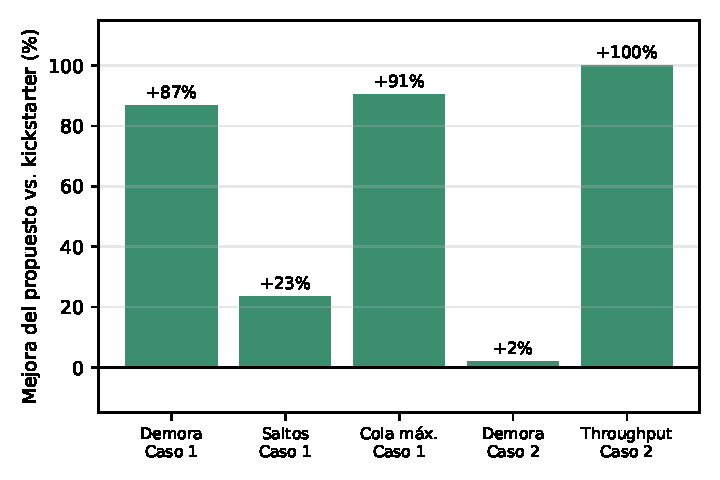
\includegraphics[width=\linewidth]{figuras/fig-comparacion-mejoras.pdf}
  \caption{Mejora porcentual del algoritmo propuesto frente al kickstarter
  (datos de la Tabla~\ref{tab:mejoras}). Barras verdes: mejora; el valor
  cercano a 0\% de ``Demora Caso 2'' se discute en el texto.}
  \label{fig:comparacion-barras}
\end{figure}

\subsection{Discusión de resultados}

\textbf{Caso 1 (escenario liviano, $\rho < 1$).} Las mejoras son grandes y
consistentes en las cuatro métricas (Tabla~\ref{tab:mejoras},
Fig.~\ref{fig:comparacion-barras}): la demora media cae 87\% (de 51.16\,s a
6.85\,s), el conteo de saltos 23\% (de 3.92 a un valor \emph{constante} de 3,
igual al óptimo) y la ocupación máxima del cuello de botella 91\% (de 190 a 18
paquetes). Es exactamente lo esperable de elegir el camino más corto: al evitar
el punto de fusión identificado en la Sección~\ref{sec:analisis}
(Fig.~\ref{fig:caso1-demora}), cada flujo circula por su propio
semianillo con carga ofrecida $\rho \approx 1$ en lugar de $\rho \approx 2$, y
el sistema deja de estar saturado.

\textbf{Caso 2 (escenario saturado, $\rho \gg 1$).} Acá conviene mirar con
cuidado: la demora media \emph{casi no cambia} ($-2\%$, de 64.53\,s a
63.35\,s). No es un fracaso del algoritmo, sino consecuencia directa de que a
\texttt{interArrivalTime} = 1\,s \emph{ambas} redes siguen sobrecargadas ---
ninguna alcanza régimen estacionario en 200\,s, y en saturación la demora está
dominada por el tiempo de cola acumulado, que crece en los dos casos. La
métrica que sí revela la mejora es el throughput sostenido: en la misma
ventana, el algoritmo propuesto entregó 398 paquetes contra 199 del
kickstarter --- exactamente el doble (Tabla~\ref{tab:comparacion}). La razón es
estructural: el algoritmo propuesto reparte los siete flujos en las dos
direcciones según la distancia real a \texttt{node[5]} (tres hacia el sentido
horario --- \texttt{node[0]}, \texttt{node[6]}, \texttt{node[7]} --- y cuatro
hacia el antihorario --- \texttt{node[1]} a \texttt{node[4]}, con
\texttt{node[1]} resolviendo a favor de ese lado el empate que se ve en la
Tabla~\ref{tab:rutas} ---), de modo que el cuello de botella más cargado pasa
de concentrar los \emph{siete} flujos ($\rho \approx 7$) a concentrar a lo sumo
\emph{cuatro} ($\rho \approx 4$). La Fig.~\ref{fig:caso2-estabilidad} muestra el
efecto de ese cambio sobre el umbral de estabilidad: mientras el kickstarter
necesita \texttt{interArrivalTime} $\gtrsim 7$\,s (Sección~\ref{sec:caso2}), el
propuesto ya es estable desde $\approx 4$--$5$\,s --- justo donde $\rho =
4/\texttt{interArrivalTime} \approx 1$ para su peor cuello de botella. La
Fig.~\ref{fig:buffer-tiempo} lo ilustra de forma muy directa: a
\texttt{interArrivalTime} = 5\,s, la cola de \texttt{node[6].lnk[0]} crece
linealmente y sin pausa con el kickstarter, mientras que con el algoritmo
propuesto fluctúa en forma acotada alrededor de un valor pequeño --- la
diferencia entre una cola con $\rho > 1$ y una con $\rho < 1$, en una sola
figura.

\begin{figure}[!t]
  \centering
  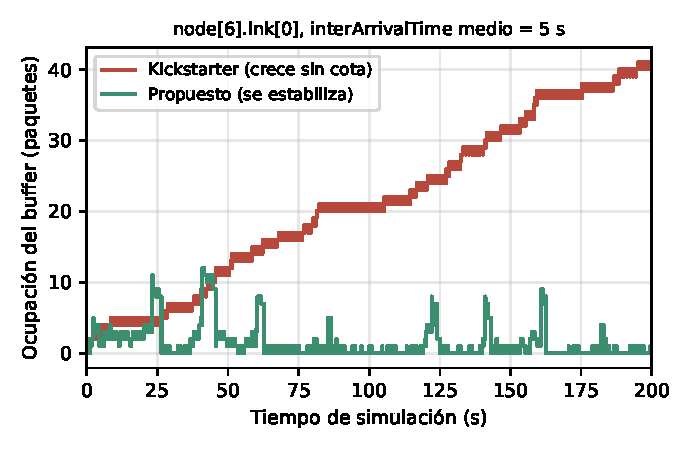
\includegraphics[width=\linewidth]{figuras/fig-buffer-tiempo.pdf}
  \caption{Ocupación de \texttt{node[6].lnk[0]} a lo largo de la simulación,
  con \texttt{interArrivalTime} medio $=5$\,s (Caso~2): el kickstarter es
  inestable en ese punto y el propuesto ya es estable.}
  \label{fig:buffer-tiempo}
\end{figure}

\textbf{¿Bucles de enrutamiento?} No observamos ninguno en ninguna corrida, y
la razón es estructural y no estadística: la regla de reenvío de
\texttt{HELLO} (``seguir por la interfaz opuesta a la de llegada, descartar al
volver al origen'') hace que cada mensaje de descubrimiento recorra el anillo
en un único sentido, sin posibilidad de ciclos; y la regla de reenvío de datos
(``ir por la interfaz de la entrada con menor cantidad de saltos'') siempre
mueve al paquete \emph{estrictamente más cerca} de su destino, porque en un
anillo las distancias por cada sentido son monótonas y nunca puede convenir
reenviar hacia un nodo que, a su vez, reenviaría de vuelta. Como verificación
indirecta: el conteo de saltos máximo que registramos para tráfico de datos con
el algoritmo propuesto, contando ambos escenarios, fue 4 (en el Caso 2; el
Caso 1 fue constante e igual a 3, Tabla~\ref{tab:comparacion}) --- igual a la
distancia máxima posible en un anillo de 8 nodos. Si hubiera bucles veríamos
conteos mucho mayores, o paquetes que nunca llegan.

\textbf{¿Y con muchos más nodos?} El tamaño de la tabla de rutas crece
linealmente con la cantidad de nodos $N$ (una entrada por destino), igual que
en cualquier protocolo de vector de distancias, y el costo de la inundación de
\texttt{HELLO} también es lineal en $N$ (cada paquete recorre el anillo una
vez). Lo que cambiaría es la \emph{ventaja relativa}: cuantos más nodos tenga
el anillo, mayor es la diferencia entre el camino más corto y el camino fijo
por \texttt{lnk[0]} (en el peor caso el kickstarter recorre $N-1$ saltos donde
el camino más corto recorre $N/2$), así que esperaríamos que la mejora en
demora y saltos \emph{crezca} con $N$, no que se diluya. El algoritmo de la
cátedra --- que entendemos apunta a generalizar a topologías arbitrarias ---
probablemente escale mejor que el nuestro en redes que no son anillos, donde
nuestra regla de terminación (``seguir por la interfaz opuesta'') deja de tener
sentido.

\textbf{¿Y si se cae un nodo?} Ninguno de los dos algoritmos lo tolera bien tal
como están. El kickstarter no tiene forma de detectarlo: seguiría reenviando
por \texttt{lnk[0]} hacia un enlace roto indefinidamente. El nuestro está
mejor posicionado \emph{en principio} --- ya cuenta con un mecanismo periódico
de descubrimiento (\texttt{helloInterval}) que, en teoría, podría notar que
dejaron de llegar \texttt{HELLO} desde cierta dirección y purgar esas rutas ---
pero en la implementación actual no lo hace: las entradas de
\texttt{routingTable} no expiran, así que si la única ruta conocida hacia un
destino deja de existir, el nodo seguiría enviando paquetes hacia un enlace
caído para siempre. Agregar una marca de tiempo a cada entrada y descartar las
que no se refrescaron en, digamos, $2\times\texttt{helloInterval}$ es una
extensión natural y relativamente sencilla sobre la base que ya construimos,
pero quedó fuera del alcance de este informe por una cuestión de tiempo.

\section{Conclusiones}
\label{sec:conclusiones}

El análisis del kickstarter (Sección~\ref{sec:analisis}) mostró que su regla
fija ``siempre por \texttt{lnk[0]}'' concentra todo el tráfico en un mismo
sentido del anillo: en el Caso~1 esto crea un punto de fusión con carga
ofrecida $\rho \approx 2$ que casi duplica la demora del tráfico que lo
atraviesa (Tabla~\ref{tab:caso1}, Fig.~\ref{fig:caso1-demora}), y en el Caso~2
concentra los siete flujos en un único cuello de botella con $\rho \approx 7$,
que se vuelve inestable a partir de \texttt{interArrivalTime} $\approx 7$\,s
(Fig.~\ref{fig:caso2-estabilidad}). A partir de ese diagnóstico diseñamos un
algoritmo de enrutamiento por camino más corto (Sección~\ref{sec:diseno}) que
construye su tabla de rutas inundando paquetes \texttt{HELLO} --- la única vía
permitida para descubrir la topología sin recorrer \texttt{cTopology} ni
\texttt{cGate} --- y reenvía cada paquete de datos por la interfaz que minimiza
la distancia conocida al destino. Activarlo con un solo parámetro
(\texttt{useShortestPath}) sobre exactamente el mismo tráfico, canales y
semilla nos permitió aislar el efecto de la decisión de enrutamiento: redujo la
demora media del Caso~1 en 87\% y la ocupación máxima de buffers en 91\%
(Tabla~\ref{tab:mejoras}), y en el Caso~2 --- donde ambas redes siguen
saturadas y la demora deja de ser el indicador relevante --- duplicó el
throughput sostenido (199 a 398 paquetes en 200\,s) y bajó el umbral de
estabilidad de $\approx 7$\,s a $\approx 4$--$5$\,s
(Fig.~\ref{fig:caso2-estabilidad}, Fig.~\ref{fig:buffer-tiempo}). No
observamos bucles de enrutamiento en ninguna corrida, y pudimos justificarlo de
forma estructural --- no sólo empírica --- a partir de las dos reglas de
reenvío del algoritmo (Sección~\ref{sec:evaluacion}).

Dicho esto, nuestra solución tiene límites que conviene dejar explícitos. Las
dos reglas que la hacen simple y liviana --- terminar la inundación de
\texttt{HELLO} por ``la interfaz opuesta'' y resolver activación de interfaces
asumiendo grado~2 --- son específicas de un anillo, y no se trasladan
directamente a topologías arbitrarias como \texttt{NetworkStar}.
Tampoco maneja caídas de nodos: las entradas de
\texttt{routingTable} no expiran, así que una ruta rota seguiría usándose para
siempre. Como trabajo futuro proponemos, en ese orden de prioridad: (1)
reemplazar la terminación ``por interfaz opuesta'' por inundación clásica con
números de secuencia, lo que generaliza el descubrimiento a cualquier
topología; y (2) agregar una marca de tiempo a cada ruta y descartar las que no
se refrescan en $2\times\texttt{helloInterval}$, para tolerar fallas de
enlaces y nodos sin rediseñar el resto del algoritmo.

\section*{Agradecimientos}

Agradecemos a la cátedra de Redes y Sistemas Distribuidos por el código base
(kickstarter) y la guía de la consigna, que nos ahorraron buena parte del
trabajo de modelado en OMNeT++ y nos dejaron concentrarnos en el diseño del
algoritmo y en el análisis de los resultados.

% Bibliografía mínima de ejemplo
\begin{thebibliography}{99}

\bibitem{omnetpp}
A. Varga and R. Hornig,
``OMNeT++,''
in \emph{Proc.\ Int.\ Conf.\ Simulation Tools and Techniques (Simutools)}, 2008.

\bibitem{kickstarter}
Cátedra de Redes y Sistemas Distribuidos,
``Laboratorio 4: kickstarter OMNeT++,''
FaMAF/UNC, 2026.

\bibitem{tanenbaum}
A. S. Tanenbaum and D. J. Wetherall,
\emph{Computer Networks}, 5th ed.
Upper Saddle River, NJ, USA: Prentice Hall, 2011.

\end{thebibliography}

\end{document}
